\section{Kết quả (Results)}
\label{sec:results}

\subsection{Phase 1 --- Base retrieval}
\label{sec:results:base}
Bảng~\ref{tab:base} cho thấy BM25 là một baseline top-rank mạnh. Dense/SciNCL cải thiện $\rechun$ so với
BM25 nhưng yếu hơn ở top-10 ranking. Hybrid RRF cho base $\ndcg$ và $\rechun$ tốt nhất, khiến nó trở thành
một candidate generator high-recall mạnh (trả lời \textbf{RQ1}).

\begin{table}[h]
\centering
\caption{Phase~1 base retrieval trên SciFact test (300 queries).}
\label{tab:base}
\begin{tabular}{llrrrr}
\toprule
Method & Model / Config & $\ndcg$ & $\recten$ & $\rechun$ & $\mrr$ \\
\midrule
BM25       & lexical, top-100             & 0.6523 & 0.7757 & 0.8731 & \textbf{0.6184} \\
Dense      & \texttt{malteos/scincl}      & 0.5640 & 0.7233 & 0.9082 & 0.5224 \\
Hybrid RRF & BM25 + SciNCL, $k{=}60$      & \textbf{0.6583} & \textbf{0.8146} & \textbf{0.9560} & 0.6157 \\
\bottomrule
\end{tabular}
\end{table}

\subsection{Dense model ablation}
\label{sec:results:dense-ablation}
Bảng~\ref{tab:dense-ablation}: SPECTER hoạt động kém trong setup này dù được thiết kế cho biểu diễn tài
liệu khoa học. MiniLM dense retrieval đáng ngạc nhiên là cạnh tranh, nhưng biến thể Hybrid RRF của nó kém
hơn hybrid SciNCL chính. Do đó dự án giữ SciNCL làm dense baseline khoa học chính.

\begin{table}[h]
\centering
\caption{Dense-encoder ablation trên SciFact test.}
\label{tab:dense-ablation}
\begin{tabular}{llrrrr}
\toprule
Method & Dense Model & $\ndcg$ & $\recten$ & $\rechun$ & $\mrr$ \\
\midrule
Dense      & \texttt{allenai/specter}                       & 0.3523 & 0.5004 & 0.7552 & 0.3133 \\
Hybrid RRF & BM25 + SPECTER                                 & 0.3863 & 0.5562 & 0.7804 & 0.3421 \\
Dense      & \texttt{all-MiniLM-L6-v2}                      & 0.6451 & 0.7833 & 0.9250 & 0.6047 \\
Hybrid RRF & BM25 + MiniLM                                  & 0.4683 & 0.7102 & 0.9120 & 0.3987 \\
\bottomrule
\end{tabular}
\end{table}

\subsection{RRF parameter ($k$) ablation}
\label{sec:results:rrf}
Bảng~\ref{tab:rrf} quét tham số $\texttt{rrf\_k}$ bằng cách re-fuse lại run BM25 và Dense đã có (không
chạy lại retrieval). Phát hiện đáng chú ý: default phổ biến $k=60$ \emph{không} tối ưu cho nDCG@10 ---
$k$ nhỏ (đặc biệt $k=5$) đặt nhiều trọng số hơn vào top-rank và đạt $\ndcg = 0.6809$, cao hơn $k=60$
($0.6583$) tới $+0.0226$. $\rechun$ không đổi ($0.9560$) ở mọi $k$ vì fusion chỉ sắp xếp lại cùng một
candidate pool. Pipeline chính vẫn giữ $k=60$ để mọi thí nghiệm Phase~3 (Always-Rerank, threshold
ablation, conformal) nhất quán trên một base ordering; nhưng ablation này cho thấy một cải thiện ``rẻ''
chưa khai thác cho base retriever, và bác bỏ giả định rằng $k=60$ là tối ưu.

\begin{table}[h]
\centering
\caption{RRF $k$ ablation trên SciFact test (re-fusion của BM25 + Dense/SciNCL). $\rechun$ không đổi vì
candidate pool giống nhau.}
\label{tab:rrf}
\begin{tabular}{rrrrr}
\toprule
$\texttt{rrf\_k}$ & $\ndcg$ & $\recten$ & $\rechun$ & $\mrr$ \\
\midrule
1            & 0.6762 & 0.8329 & 0.9560 & 0.6295 \\
5            & \textbf{0.6809} & 0.8339 & 0.9560 & \textbf{0.6358} \\
10           & 0.6773 & \textbf{0.8398} & 0.9560 & 0.6316 \\
20           & 0.6710 & 0.8354 & 0.9560 & 0.6249 \\
40           & 0.6613 & 0.8204 & 0.9560 & 0.6175 \\
60 (default) & 0.6583 & 0.8146 & 0.9560 & 0.6157 \\
80           & 0.6557 & 0.8079 & 0.9560 & 0.6143 \\
100          & 0.6554 & 0.8079 & 0.9560 & 0.6139 \\
200          & 0.6555 & 0.8079 & 0.9560 & 0.6140 \\
\bottomrule
\end{tabular}
\end{table}

\subsection{Phase 2 --- Router results}
\label{sec:results:router}
Bảng~\ref{tab:router} cho thấy oracle có headroom đáng kể ($\ndcg = 0.7617$ so với $0.6583$ của Hybrid),
trả lời \textbf{RQ2}. Tuy nhiên Majority Router khó vượt vì test labels thiên mạnh về BM25. Small LLM
router thô cải thiện đáng kể sau khi chuyển sang label log-probability scoring, nhưng vẫn dưới Majority
Router trên toàn bộ 300 query; calibrated held-out route nâng $\ndcg$ lên $0.6674$ trên 150 held-out
query (trả lời một phần \textbf{RQ3}, \textbf{RQ4}).

\begin{table}[h]
\centering
\caption{Phase~2 router results trên SciFact test. Oracle là upper bound. Classical TF-IDF router và LLM
router đều train trên \emph{train} split, đánh giá trên \emph{test} split (không leakage). Calibrated
route đánh giá trên 150 held-out query (xem Phần~\ref{sec:results:heldout} để so sánh công bằng).}
\label{tab:router}
\setlength{\tabcolsep}{4.5pt}
\begin{tabular}{lrrrrrr}
\toprule
Router & Acc. & Macro-F1 & $\ndcg$ & $\recten$ & $\rechun$ & $\mrr$ \\
\midrule
Random Router                       & 0.3267 & 0.2617 & 0.6290 & 0.7778 & 0.9132 & 0.5875 \\
Majority Router                     & 0.7533 & 0.2864 & 0.6523 & 0.7757 & 0.8731 & 0.6184 \\
Oracle Router                       & 1.0000 & 1.0000 & \textbf{0.7617} & \textbf{0.8711} & 0.9127 & \textbf{0.7337} \\
Classical TF-IDF LogReg             & 0.2867 & 0.2504 & 0.6368 & 0.8144 & 0.9216 & 0.5880 \\
Small LLM QLoRA (LogProb)           & 0.4300 & 0.3076 & 0.6372 & 0.7788 & 0.9046 & 0.5980 \\
Small LLM QLoRA (Calibrated H.O.)   & 0.3133 & 0.2097 & 0.6674 & 0.8161 & 0.8947 & 0.6259 \\
\bottomrule
\end{tabular}
\end{table}

Lưu ý quan trọng khi đọc bảng: \emph{accuracy thấp không đồng nghĩa retrieval kém}. Classical TF-IDF
router (trained on train, eval on test) chỉ đạt accuracy 0.287 --- thấp hơn cả Majority Router --- nhưng
$\ndcg = 0.6368$ của nó vẫn ngang với Small LLM router (0.6372), vì khi route ``sai'' nhãn oracle nó
thường chọn một route vẫn xếp hạng tốt. Đây chính là động lực cho \emph{Mean Regret@10}
(Phần~\ref{sec:results:heldout}): hai learned router (classical và LLM) độc lập nhau đều bị
train/test distribution shift kéo accuracy xuống, nhưng tổn thất retrieval thực tế nhỏ hơn nhiều. Vì cùng
lý do, calibrated route có accuracy thấp nhất (0.313) nhưng $\ndcg$ cao nhất trong nhóm learned
(0.6674): calibration tối ưu retrieval quality chứ không tối ưu khớp nhãn oracle.

Trong các phiên bản trước, classical router từng được train và evaluate trên \emph{cùng} test split, cho
kết quả in-split phi thực tế (Acc.~$=0.9933$, $\ndcg = 0.7617$). Kết quả leaky này đã được thay bằng
setup train$\to$test ở trên; nó chỉ còn ý nghĩa như một sanity check rằng bài toán route-label là học
được, không phải một baseline hợp lệ.

\subsection{So sánh công bằng trên held-out subset}
\label{sec:results:heldout}
Calibrated LLM route được đánh giá trên 150 held-out query (chọn bằng \texttt{seed=13} sau khi dùng 150
query còn lại cho calibration). Bảng~\ref{tab:heldout} đánh giá BM25, Dense, Hybrid và calibrated route
trên \emph{đúng} subset này. \emph{Mean Regret@10} được định nghĩa là oracle per-query $\ndcg$ trừ
per-query $\ndcg$ của route được chọn, trung bình trên subset --- một thước đo hữu ích vì label accuracy
có thể gây hiểu nhầm: chọn một route khác có thể gần như không phạt nếu hai route xếp hạng tài liệu liên
quan tương tự.

\begin{table}[h]
\centering
\caption{So sánh công bằng trên 150 held-out query. Calibrated route có Mean Regret@10 thấp nhất và
$\ndcg$/$\mrr$ tốt nhất, nhưng Hybrid RRF vẫn có $\rechun$ tốt nhất.}
\label{tab:heldout}
\setlength{\tabcolsep}{4.5pt}
\begin{tabular}{lrrrrrr}
\toprule
Method & Queries & $\ndcg$ & $\recten$ & $\rechun$ & $\mrr$ & Mean Regret@10 \\
\midrule
BM25                       & 150 & 0.6489 & 0.7656 & 0.8691 & 0.6184 & 0.0893 \\
Dense/SciNCL               & 150 & 0.5063 & 0.6491 & 0.8887 & 0.4690 & 0.2319 \\
Hybrid RRF                 & 150 & 0.6357 & 0.8028 & \textbf{0.9387} & 0.5884 & 0.1025 \\
Small LLM Calibrated H.O.  & 150 & \textbf{0.6674} & \textbf{0.8161} & 0.8947 & \textbf{0.6259} & \textbf{0.0708} \\
\bottomrule
\end{tabular}
\end{table}

\subsection{So sánh Quality-vs-Cost}
\label{sec:results:costquality}
Bảng~\ref{tab:costquality} tổng hợp đánh đổi cost--quality (trả lời \textbf{RQ5}). BM25 là baseline
low-cost mạnh nhất; Hybrid RRF cải thiện recall ở chi phí cao hơn; routing LLM thô hạ chi phí ước tính so
với luôn dùng Hybrid nhưng mất $\ndcg$; calibrated fallback cải thiện route LLM nhưng tăng chi phí vì nhiều
query uncertain rơi về Hybrid. Các hàng có số query khác nhau không hoàn toàn so sánh được; so sánh
effectiveness công bằng cho calibrated route là Bảng~\ref{tab:heldout}.

\begin{table}[h]
\centering
\caption{Bảng cost--quality (cost unit trừu tượng của Phase~2). Các hàng khác số query không hoàn toàn
so sánh được về effectiveness.}
\label{tab:costquality}
\setlength{\tabcolsep}{3.5pt}
\small
\begin{tabular}{lrrlrrrr}
\toprule
Method & \#Q & Cost/Q & Route dist. & $\ndcg$ & $\recten$ & $\rechun$ & $\mrr$ \\
\midrule
BM25                    & 300 & 1.00 & bm25                    & 0.6523 & 0.7757 & 0.8731 & 0.6184 \\
Dense                   & 300 & 3.00 & dense                   & 0.5640 & 0.7233 & 0.9082 & 0.5224 \\
Hybrid RRF              & 300 & 4.00 & hybrid                  & 0.6583 & 0.8146 & 0.9560 & 0.6157 \\
LLM QLoRA LogProb       & 300 & 2.31 & b113/d169/h18           & 0.6372 & 0.7788 & 0.9046 & 0.5980 \\
LLM QLoRA Calib. H.O.   & 150 & 3.16 & b42/h108                & 0.6674 & 0.8161 & 0.8947 & 0.6259 \\
\bottomrule
\end{tabular}
\end{table}

\subsection{Phase 3 --- Always-Rerank baseline}
\label{sec:results:alwaysrerank}
Baseline Always-Rerank rerank Hybrid RRF top-20 cho tất cả 300 test query bằng cross-encoder
\texttt{ms-marco-MiniLM-L-6-v2} trên một GPU RTX~5070~Ti (Bảng~\ref{tab:alwaysrerank}). Nó cải thiện
$\ndcg$ thêm $+0.0356$ và $\mrr$ thêm $+0.0447$ so với Hybrid RRF. $\rechun$ giữ nguyên ở $0.9560$ vì
reranking chỉ sắp xếp lại tập top-20 sẵn có chứ không thêm document mới vào pool top-100. Kết quả reranked
vẫn dưới Oracle Router, để lại chỗ cho selective reranking tiệm cận chất lượng Always-Rerank ở chi phí thấp
hơn. Đây là kết quả Phase~3 đầu tiên dùng wall-clock latency đo thực thay cho cost unit trừu tượng.

\begin{table}[h]
\centering
\caption{Phase~3 Always-Rerank baseline (Hybrid top-20, MiniLM-L-6-v2) trên SciFact test.}
\label{tab:alwaysrerank}
\setlength{\tabcolsep}{4pt}
\begin{tabular}{lrrrrrr}
\toprule
Method & $\ndcg$ & $\recten$ & $\rechun$ & $\mrr$ & Cov. & ms/query \\
\midrule
Hybrid RRF (base)              & 0.6583 & 0.8146 & 0.9560 & 0.6157 & 0.00 & n/a \\
Always-Rerank (Hybrid top-20)  & \textbf{0.6939} & \textbf{0.8286} & 0.9560 & \textbf{0.6604} & 1.00 & 27.3 \\
Oracle Router (reference)      & 0.7617 & 0.8711 & 0.9127 & 0.7337 & n/a & n/a \\
\bottomrule
\end{tabular}
\end{table}

\subsection{Selective reranking --- Threshold ablation}
\label{sec:results:ablation}
Bảng~\ref{tab:table3} báo cáo đánh đổi full-test. Headline selective point là ngưỡng score-gap coverage
nhỏ nhất thu lại ít nhất 90\% lợi ích $\ndcg$ của Always-Rerank.

\begin{table}[h]
\centering
\caption{Phase~3 effectiveness-vs-cost trên SciFact test (300 queries). $\rechun$ không đổi ở $0.9560$ vì
reranking chỉ sắp xếp lại top-20 sẵn có.}
\label{tab:table3}
\setlength{\tabcolsep}{4pt}
\begin{tabular}{lrrrrrr}
\toprule
Method & $\ndcg$ & $\recten$ & $\rechun$ & $\mrr$ & Cov. & ms/query \\
\midrule
BM25                                       & 0.6523 & 0.7757 & 0.8731 & 0.6184 & 0.00 & 0.0 \\
Dense / SciNCL                             & 0.5640 & 0.7233 & 0.9082 & 0.5224 & 0.00 & 0.0 \\
Hybrid RRF                                 & 0.6583 & 0.8146 & 0.9560 & 0.6157 & 0.00 & 0.0 \\
Selective rerank (score-gap, headline)     & 0.6924 & 0.8186 & 0.9560 & 0.6611 & 0.66 & 18.1 \\
Selective rerank (config-default OR-rule)  & \textbf{0.6977} & 0.8286 & 0.9560 & \textbf{0.6649} & 0.82 & 22.5 \\
Always-Rerank                              & 0.6939 & 0.8286 & 0.9560 & 0.6604 & 1.00 & 27.3 \\
\bottomrule
\end{tabular}
\end{table}

\begin{figure}[h]
\centering
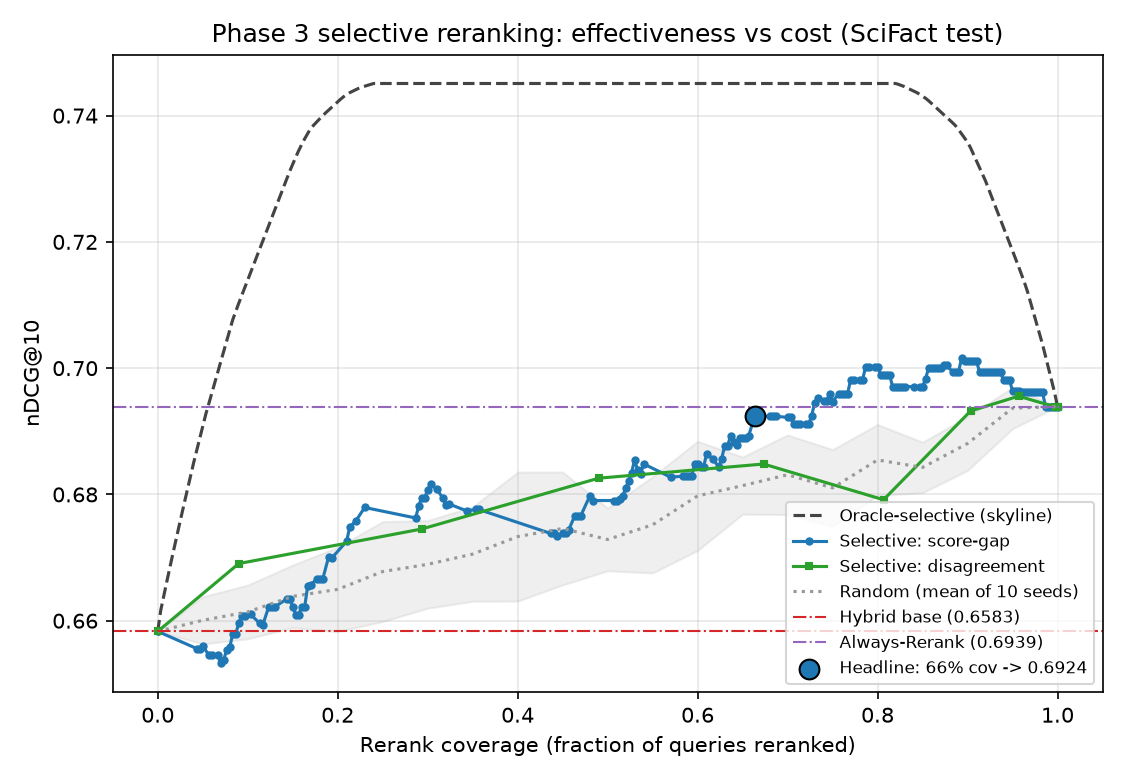
\includegraphics[width=0.82\textwidth]{figures/phase3_pareto.png}
\caption{$\ndcg$ theo rerank coverage. Oracle-selective skyline đạt $\ndcg \approx 0.745$ ở khoảng 25\%
coverage, nhưng hai tín hiệu label-free (score gap, disagreement) bám sát baseline random.}
\label{fig:pareto}
\end{figure}

Ba phát hiện nổi bật. \emph{Thứ nhất}, các tín hiệu uncertainty hiện tại chỉ informative ở mức biên: diện
tích dưới đường cong nDCG-vs-coverage là $0.6814$ cho score gap và $0.6795$ cho disagreement, chỉ nhỉnh
hơn baseline random $0.6753$, và thấp hơn nhiều so với oracle-selective skyline $0.7350$. Khoảng cách
skyline lớn này cho thấy có headroom thực cho một tín hiệu trigger tốt hơn, trực tiếp thúc đẩy nâng cấp
sang QPP và conformal (Phần~\ref{sec:results:qpp}--\ref{sec:results:conformal}). \emph{Thứ hai}, config-default
OR rule ban đầu (\texttt{score\_gap < 0.03} OR \texttt{disagreement > 0.85}) quá dễ kích hoạt nên rerank
mọi query và sụp về Always-Rerank; sau khi chỉnh default về ngưỡng đã tune trên held-out
(\texttt{score\_gap < 0.0024} OR \texttt{disagreement > 0.95}), nó rerank 82\% query và đạt $\ndcg = 0.6977$
ở 22.5~ms/query --- \emph{cao hơn} cả Always-Rerank. \emph{Thứ ba}, đây cũng cho thấy selective reranking
có thể \emph{nhỉnh hơn} Always-Rerank quanh 80\% coverage, vì reranking thực sự làm \emph{hại} một thiểu số
query và bỏ qua chúng lấy lại được chút chất lượng.

Để tránh chọn ngưỡng trên cùng query dùng để đánh giá, Bảng~\ref{tab:table3b} tune ngưỡng score-gap trên
150 calibration query (\texttt{seed=13}) và báo cáo trên 150 evaluation query rời rạc.

\begin{table}[h]
\centering
\caption{Selective reranking held-out không rò rỉ. Ngưỡng score-gap tune trên calibration; selective
reranking đạt $\ndcg = 0.7145$ ở 74\% coverage trên evaluation, thu lại phần lớn lợi ích của Always-Rerank
($0.7181$) ở khoảng ba phần tư chi phí.}
\label{tab:table3b}
\setlength{\tabcolsep}{4pt}
\begin{tabular}{lrrrrrr}
\toprule
Method (eval subset) & $\ndcg$ & $\recten$ & $\rechun$ & $\mrr$ & Cov. & ms/query \\
\midrule
Hybrid RRF (no rerank)               & 0.6860 & 0.8311 & 0.9787 & 0.6457 & 0.00 & 0.0 \\
Selective rerank (held-out tuned)    & 0.7145 & 0.8224 & 0.9787 & 0.6892 & 0.74 & 20.2 \\
Always-Rerank                        & \textbf{0.7181} & \textbf{0.8358} & 0.9787 & \textbf{0.6907} & 1.00 & 27.3 \\
\bottomrule
\end{tabular}
\end{table}

\subsection{QPP signals cho rerank trigger}
\label{sec:results:qpp}
Bảng~\ref{tab:qpp} cho thấy Hybrid maximum RRF score là tín hiệu informative nhất. Nó tương quan mạnh và
dương với base $\ndcg$ (Kendall $+0.500$): khi top fused score cao, kết quả un-reranked vốn đã tốt. Do đó
nó có tương quan âm mạnh nhất với gain-from-reranking (Kendall $-0.166$, gần ba lần $-0.060$ của score
gap): một max score thấp gắn cờ một base result yếu nơi reranking có khả năng giúp nhất. Các tín hiệu còn
lại, gồm cả score gap của Phase~3, chỉ tương quan yếu với gain. Điều này khớp với phát hiện rộng hơn rằng
QPP cho dense và fused retrieval là khó, nhưng nó xác định một trigger rõ ràng tốt hơn heuristic ban đầu.

\begin{table}[h]
\centering
\caption{Kendall correlation của các QPP signal chọn lọc với base quality và gain-from-reranking (SciFact
test; bảng đầy đủ ở \texttt{reports/tables/qpp\_correlations.md}).}
\label{tab:qpp}
\begin{tabular}{lrr}
\toprule
Feature & Kendall vs base nDCG & Kendall vs gain-from-rerank \\
\midrule
Hybrid max score             & $+0.500$ & $\mathbf{-0.166}$ \\
Dense NQC / std              & $+0.240$ & $-0.090$ \\
Hybrid score gap (Phase 3)   & $+0.112$ & $-0.060$ \\
BM25--Dense disagreement     & $-0.134$ & $+0.029$ \\
\bottomrule
\end{tabular}
\end{table}

\begin{figure}[h]
\centering
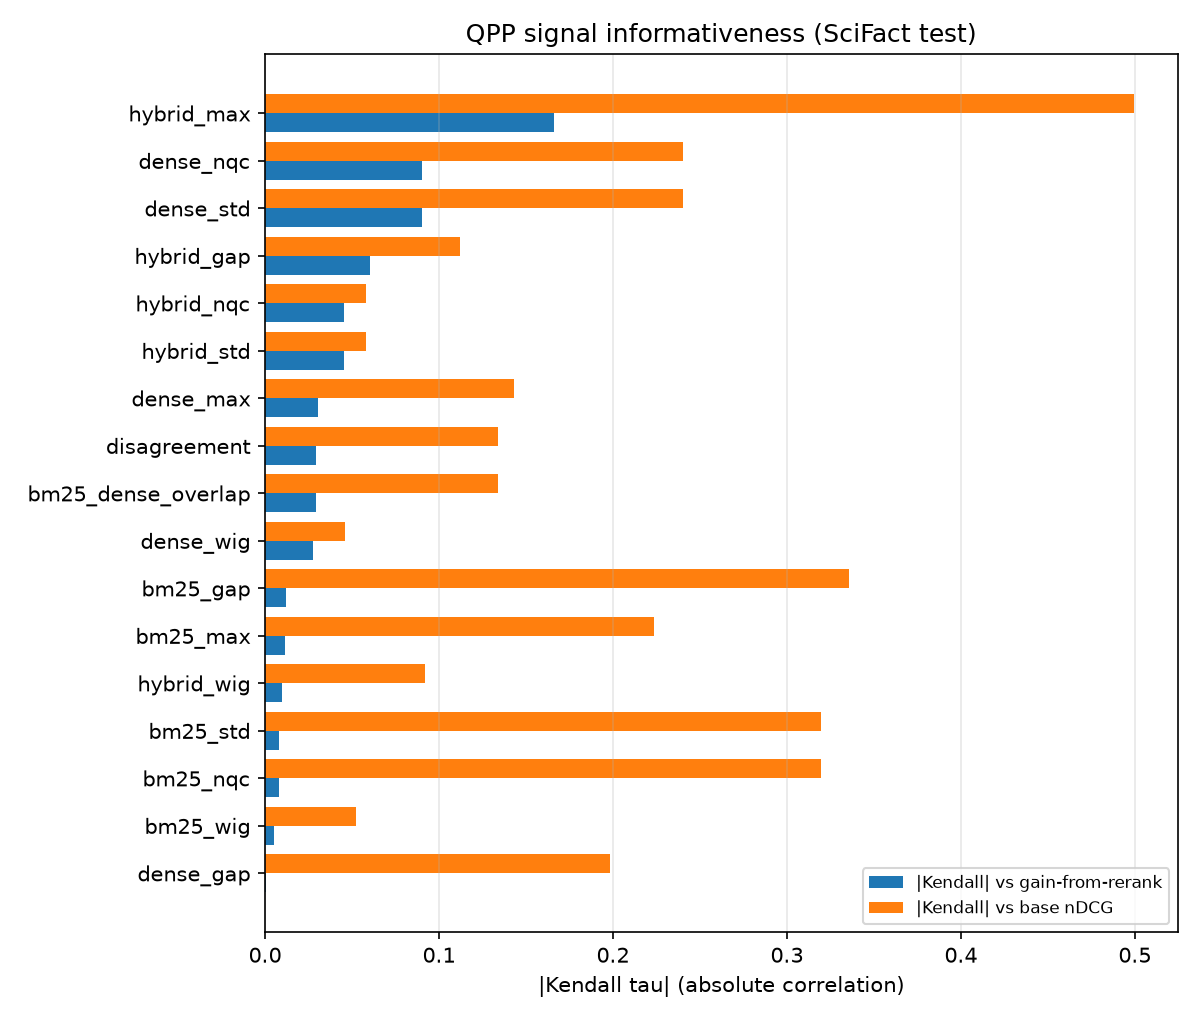
\includegraphics[width=0.82\textwidth]{figures/qpp_correlations.png}
\caption{Tương quan của các QPP predictor với base $\ndcg$ và gain-from-reranking. Hybrid max score là
predictor mạnh nhất cho cả hai target.}
\label{fig:qpp}
\end{figure}

\subsection{Conformal risk-controlled selective reranking}
\label{sec:results:conformal}
Chúng tôi chạy CRC với QPP signal (Hybrid max score) và, để so sánh, với Phase~3 score gap; tune trên 150
calibration query và evaluate trên 150 query rời rạc. Bảng~\ref{tab:conformal} báo cáo operating point ở
$\alpha = 0.02$.

\begin{table}[h]
\centering
\caption{Conformal risk-controlled selective reranking ở $\alpha = 0.02$ (eval split; Hybrid base
$\ndcg = 0.6860$, Always-Rerank $= 0.7181$).}
\label{tab:conformal}
\setlength{\tabcolsep}{5pt}
\begin{tabular}{lrrrcr}
\toprule
Trigger signal & Cov. & $\ndcg$ & Realized risk & Guarantee & ms/query \\
\midrule
QPP: Hybrid max score        & \textbf{0.61} & \textbf{0.7280} & 0.0052 & yes & \textbf{16.6} \\
Phase 3 heuristic: score gap & 0.72 & 0.7120 & 0.0152 & yes & 19.6 \\
\bottomrule
\end{tabular}
\end{table}

\begin{figure}[h]
\centering
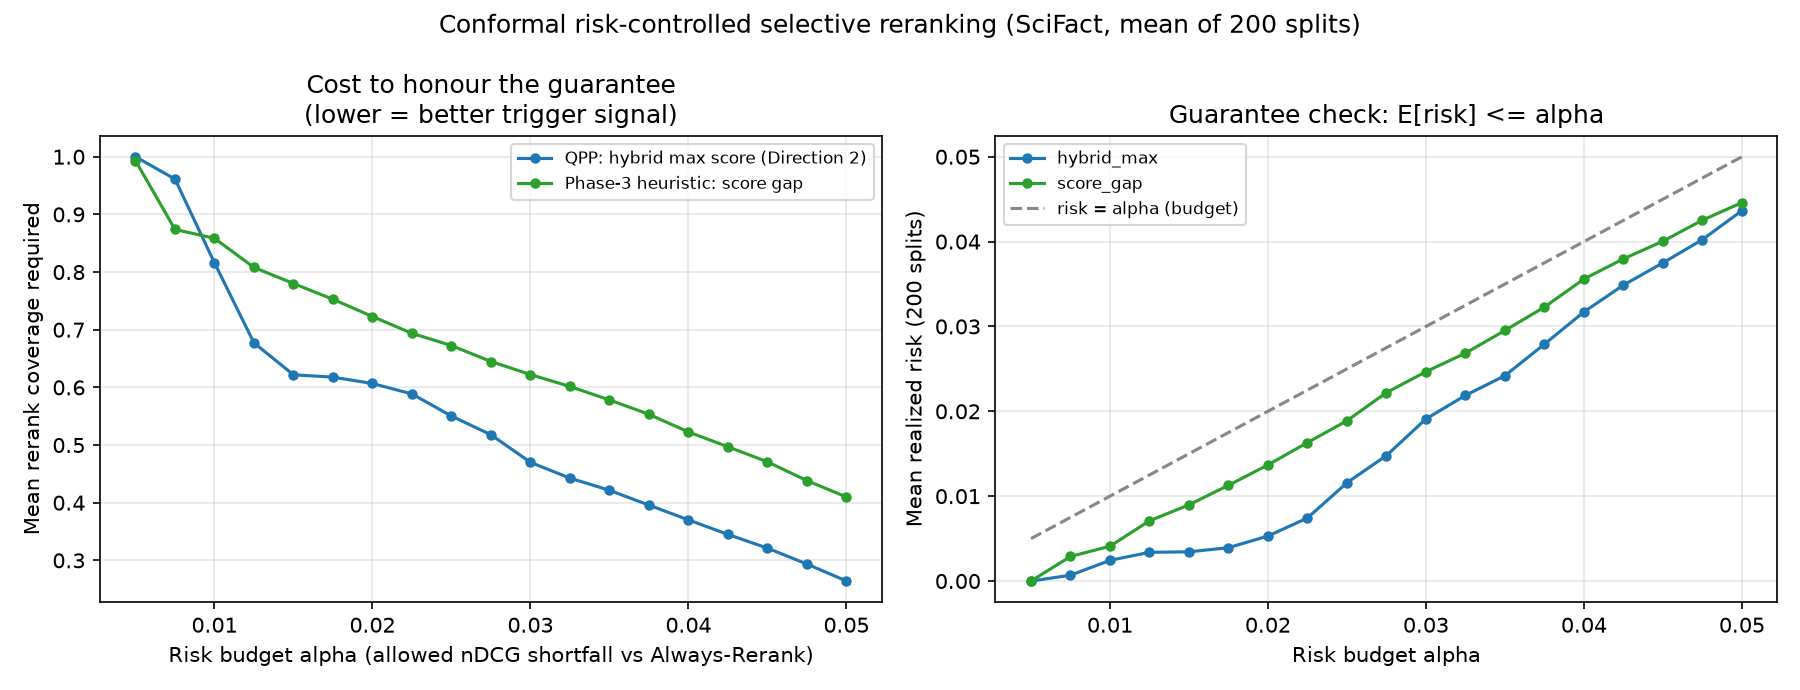
\includegraphics[width=0.92\textwidth]{figures/phase3_conformal_risk_coverage.png}
\caption{Trái: rerank coverage mà CRC yêu cầu để tôn trọng mỗi risk budget $\alpha$; tín hiệu QPP (Hybrid
max) nằm dưới heuristic score-gap ở mọi nơi, nên rẻ hơn ở mọi mức bảo đảm. Phải: realized risk trung bình
trên 200 split nằm dưới đường $\text{risk}=\alpha$, xác nhận bảo đảm.}
\label{fig:conformal}
\end{figure}

Hai kết quả nổi bật. \emph{Thứ nhất}, tín hiệu QPP tôn trọng cùng risk budget ở 61\% coverage so với 72\%
của score gap --- giảm 11 điểm chi phí reranking --- và đạt $\ndcg$ cao hơn ($0.7280$ so với $0.7120$).
Đáng chú ý $0.7280$ nhỉnh hơn Always-Rerank ($0.7181$) vì trigger bỏ qua các query mà reranking sẽ làm hại.
\emph{Thứ hai}, bảo đảm giữ vững: trung bình trên 200 calibration/evaluation split, realized risk luôn
$\le \alpha$ cho mọi budget và cả hai tín hiệu (0/38 operating point vi phạm $\mathbb{E}[\text{risk}] \le \alpha$).
Trên một split đơn lẻ, realized risk có thể vượt $\alpha$, đúng như kỳ vọng cho một bảo đảm in-expectation.

Cùng nhau, các kết quả này khép lại luận điểm cốt lõi: một tín hiệu QPP rẻ, label-free, cộng với một ngưỡng
conformal quyết định khi nào cross-encoder đắt đỏ là đáng chạy, kèm bảo đảm thống kê về chất lượng đánh đổi,
và ở coverage thấp hơn đáng kể so với heuristic ban đầu.

\subsection{Kiểm định ý nghĩa thống kê (Significance testing)}
\label{sec:results:significance}
Vì các bảng trên là point estimate, chúng tôi bổ sung \emph{paired bootstrap} trên query (10{,}000
resample, seed=13) cho các so sánh then chốt. Với mỗi cặp (system, baseline), ta tính per-query $\ndcg$ và
$\mrr$ trên tập query chung, rồi ước lượng mean paired difference cùng khoảng tin cậy 95\% và p-value hai
phía. Bảng~\ref{tab:sig} tổng hợp.

\begin{table}[h]
\centering
\caption{Paired bootstrap (10{,}000 resample). CI là khoảng 95\% của mean paired difference; in đậm khi CI
loại trừ 0 (khác biệt có ý nghĩa). ``H.O.''~$=$~held-out 150 query.}
\label{tab:sig}
\setlength{\tabcolsep}{4pt}
\small
\begin{tabular}{llrrr}
\toprule
So sánh & Metric & Mean diff & 95\% CI & p \\
\midrule
Hybrid RRF vs BM25            & $\ndcg$ & $+0.0060$ & $[-0.022, +0.034]$ & 0.665 \\
Hybrid RRF vs BM25            & $\mrr$  & $-0.0027$ & $[-0.035, +0.030]$ & 0.875 \\
Always-Rerank vs Hybrid RRF   & $\ndcg$ & $\mathbf{+0.0356}$ & $[+0.008, +0.063]$ & \textbf{0.012} \\
Always-Rerank vs Hybrid RRF   & $\mrr$  & $\mathbf{+0.0447}$ & $[+0.011, +0.080]$ & \textbf{0.009} \\
Oracle Router vs Hybrid RRF   & $\ndcg$ & $\mathbf{+0.1034}$ & $[+0.080, +0.128]$ & \textbf{<0.001} \\
Oracle Router vs Hybrid RRF   & $\mrr$  & $\mathbf{+0.1180}$ & $[+0.091, +0.147]$ & \textbf{<0.001} \\
Calibrated LLM (H.O.) vs BM25 & $\ndcg$ & $+0.0186$ & $[-0.011, +0.048]$ & 0.213 \\
Calibrated LLM (H.O.) vs BM25 & $\mrr$  & $+0.0075$ & $[-0.025, +0.040]$ & 0.640 \\
\bottomrule
\end{tabular}
\end{table}

Kết quả này định cỡ lại các tuyên bố một cách trung thực. \emph{Thứ nhất}, lợi thế $\ndcg$ của Hybrid RRF
so với BM25 \emph{không} có ý nghĩa thống kê ($p = 0.665$) --- giá trị thực của Hybrid nằm ở $\rechun$
(0.9560 vs 0.8731), tức nó là một \emph{candidate generator} tốt hơn chứ không phải một top-ranker tốt hơn.
\emph{Thứ hai}, cải thiện của Always-Rerank so với Hybrid \emph{có} ý nghĩa cho cả $\ndcg$ ($p = 0.012$) và
$\mrr$ ($p = 0.009$): đóng góp chính của Phase~3 đứng vững dưới kiểm định. \emph{Thứ ba}, headroom của
Oracle Router rất có ý nghĩa ($p < 0.001$), khẳng định dư địa routing là thật. \emph{Thứ tư}, cải thiện của
calibrated LLM route so với BM25 \emph{chưa} đạt ý nghĩa ($p = 0.213$) trên 150 query --- nhất quán với kết
luận rằng LLM router là một thành phần hữu ích nhưng chưa phải đóng góp độc lập đủ mạnh.
